% Options for packages loaded elsewhere
\PassOptionsToPackage{unicode}{hyperref}
\PassOptionsToPackage{hyphens}{url}
%
\documentclass[
  12pt,
]{article}
\usepackage{amsmath,amssymb}
\usepackage{lmodern}
\usepackage{ifxetex,ifluatex}
\ifnum 0\ifxetex 1\fi\ifluatex 1\fi=0 % if pdftex
  \usepackage[T1]{fontenc}
  \usepackage[utf8]{inputenc}
  \usepackage{textcomp} % provide euro and other symbols
\else % if luatex or xetex
  \usepackage{unicode-math}
  \defaultfontfeatures{Scale=MatchLowercase}
  \defaultfontfeatures[\rmfamily]{Ligatures=TeX,Scale=1}
\fi
% Use upquote if available, for straight quotes in verbatim environments
\IfFileExists{upquote.sty}{\usepackage{upquote}}{}
\IfFileExists{microtype.sty}{% use microtype if available
  \usepackage[]{microtype}
  \UseMicrotypeSet[protrusion]{basicmath} % disable protrusion for tt fonts
}{}
\makeatletter
\@ifundefined{KOMAClassName}{% if non-KOMA class
  \IfFileExists{parskip.sty}{%
    \usepackage{parskip}
  }{% else
    \setlength{\parindent}{0pt}
    \setlength{\parskip}{6pt plus 2pt minus 1pt}}
}{% if KOMA class
  \KOMAoptions{parskip=half}}
\makeatother
\usepackage{xcolor}
\IfFileExists{xurl.sty}{\usepackage{xurl}}{} % add URL line breaks if available
\IfFileExists{bookmark.sty}{\usepackage{bookmark}}{\usepackage{hyperref}}
\hypersetup{
  pdftitle={Stand Up Fight Back},
  pdfauthor={Kevin Morris; Kelsey Shoub},
  hidelinks,
  pdfcreator={LaTeX via pandoc}}
\urlstyle{same} % disable monospaced font for URLs
\usepackage[margin=1in]{geometry}
\usepackage{longtable,booktabs,array}
\usepackage{calc} % for calculating minipage widths
% Correct order of tables after \paragraph or \subparagraph
\usepackage{etoolbox}
\makeatletter
\patchcmd\longtable{\par}{\if@noskipsec\mbox{}\fi\par}{}{}
\makeatother
% Allow footnotes in longtable head/foot
\IfFileExists{footnotehyper.sty}{\usepackage{footnotehyper}}{\usepackage{footnote}}
\makesavenoteenv{longtable}
\usepackage{graphicx}
\makeatletter
\def\maxwidth{\ifdim\Gin@nat@width>\linewidth\linewidth\else\Gin@nat@width\fi}
\def\maxheight{\ifdim\Gin@nat@height>\textheight\textheight\else\Gin@nat@height\fi}
\makeatother
% Scale images if necessary, so that they will not overflow the page
% margins by default, and it is still possible to overwrite the defaults
% using explicit options in \includegraphics[width, height, ...]{}
\setkeys{Gin}{width=\maxwidth,height=\maxheight,keepaspectratio}
% Set default figure placement to htbp
\makeatletter
\def\fps@figure{htbp}
\makeatother
\setlength{\emergencystretch}{3em} % prevent overfull lines
\providecommand{\tightlist}{%
  \setlength{\itemsep}{0pt}\setlength{\parskip}{0pt}}
\setcounter{secnumdepth}{5}
\usepackage{rotating}
\usepackage{setspace}
\usepackage{booktabs}
\usepackage{longtable}
\usepackage{array}
\usepackage{multirow}
\usepackage{wrapfig}
\usepackage{float}
\usepackage{colortbl}
\usepackage{pdflscape}
\usepackage{tabu}
\usepackage{threeparttable}
\usepackage{threeparttablex}
\usepackage[normalem]{ulem}
\usepackage{makecell}
\usepackage{xcolor}
\ifluatex
  \usepackage{selnolig}  % disable illegal ligatures
\fi

\title{Stand Up Fight Back\thanks{Thanks.}}
\usepackage{etoolbox}
\makeatletter
\providecommand{\subtitle}[1]{% add subtitle to \maketitle
  \apptocmd{\@title}{\par {\large #1 \par}}{}{}
}
\makeatother
\subtitle{How Police Killings Can Mobilize Local Communities}
\author{Kevin Morris\footnote{Brennan Center for Justice, Researcher (\href{mailto:kevin.morris@nyu.edu}{\nolinkurl{kevin.morris@nyu.edu}})} \and Kelsey Shoub\footnote{University of South Carolina, Assistant Professor (\href{mailto:kshoub@mailbox.sc.edu}{\nolinkurl{kshoub@mailbox.sc.edu}})}}
\date{May 04, 2022}

\begin{document}
\maketitle
\begin{abstract}
TKTKTKTK
\end{abstract}

\pagenumbering{gobble}
\pagebreak
\doublespacing

\pagenumbering{arabic}

\begin{figure}[h]

{\centering 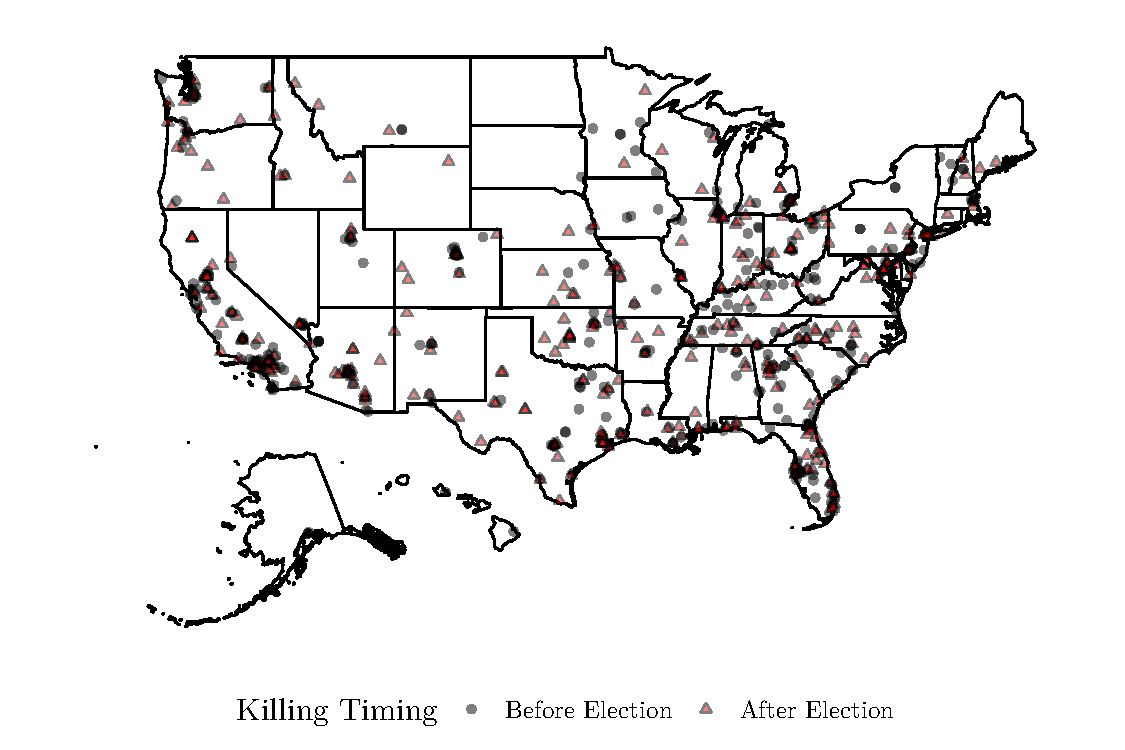
\includegraphics{shoot_to_files/figure-latex/map-1} 

}

\caption{\label{fig:map}Police Killing within 2 Months of Election, 2016 and 2020}\label{fig:map}
\end{figure}

\begin{figure}[h]

{\centering 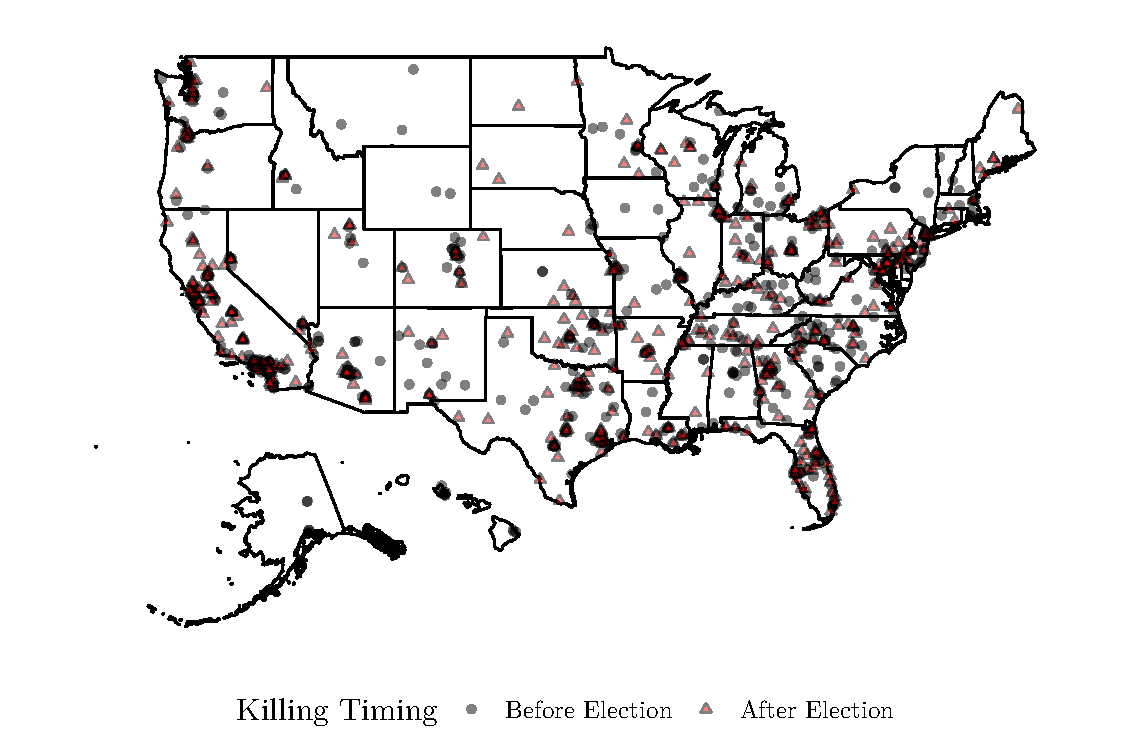
\includegraphics{shoot_to_files/figure-latex/map-16-1} 

}

\caption{\label{fig:map}Police Killing within 2 Months of Election, 2016 and 2020}\label{fig:map-16}
\end{figure}

\begin{figure}[h]

{\centering 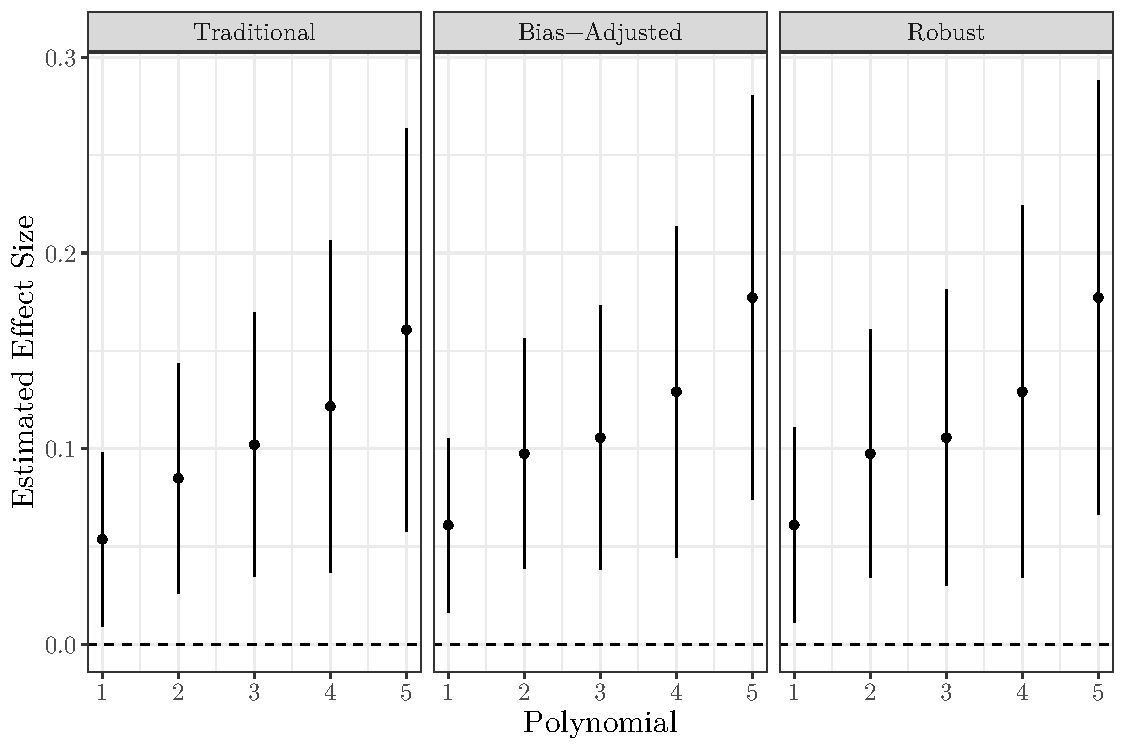
\includegraphics{shoot_to_files/figure-latex/diff-poly-1} 

}

\caption{\label{fig:map}Police Killing within 2 Months of Election, 2016 and 2020}\label{fig:diff-poly}
\end{figure}

\begin{figure}[h]

{\centering 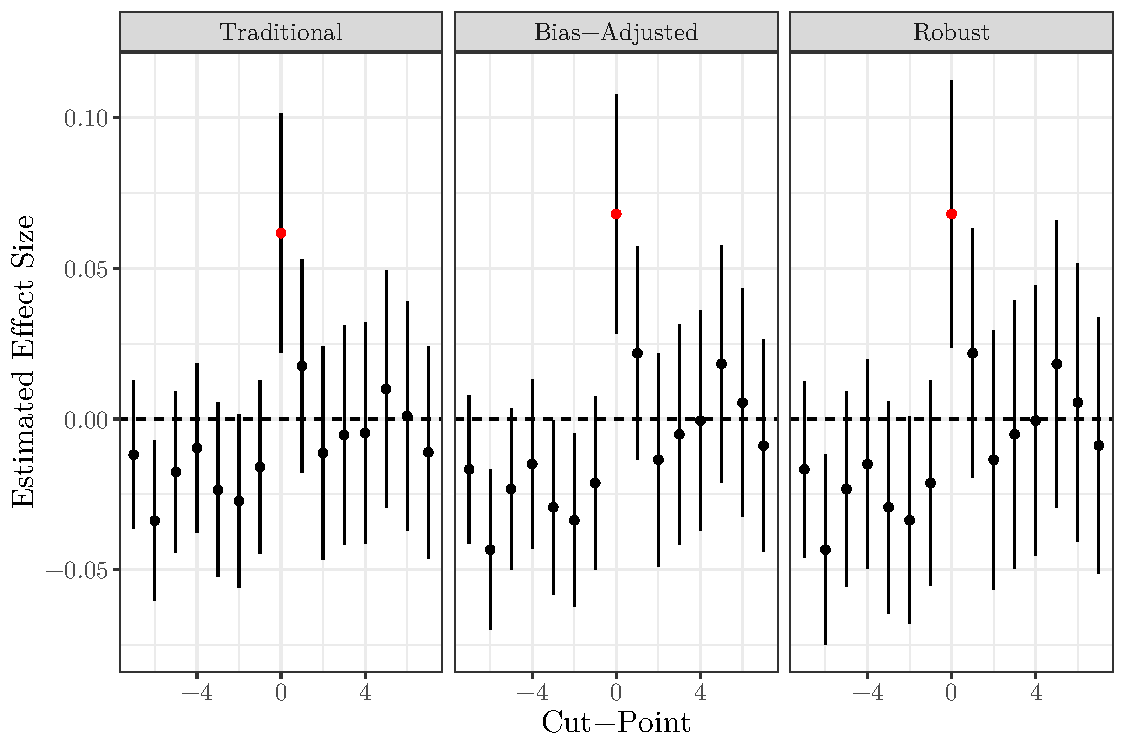
\includegraphics{shoot_to_files/figure-latex/placebo-cuts-1} 

}

\caption{\label{fig:map}Police Killing within 2 Months of Election, 2016 and 2020}\label{fig:placebo-cuts}
\end{figure}

\begin{figure}[h]

{\centering 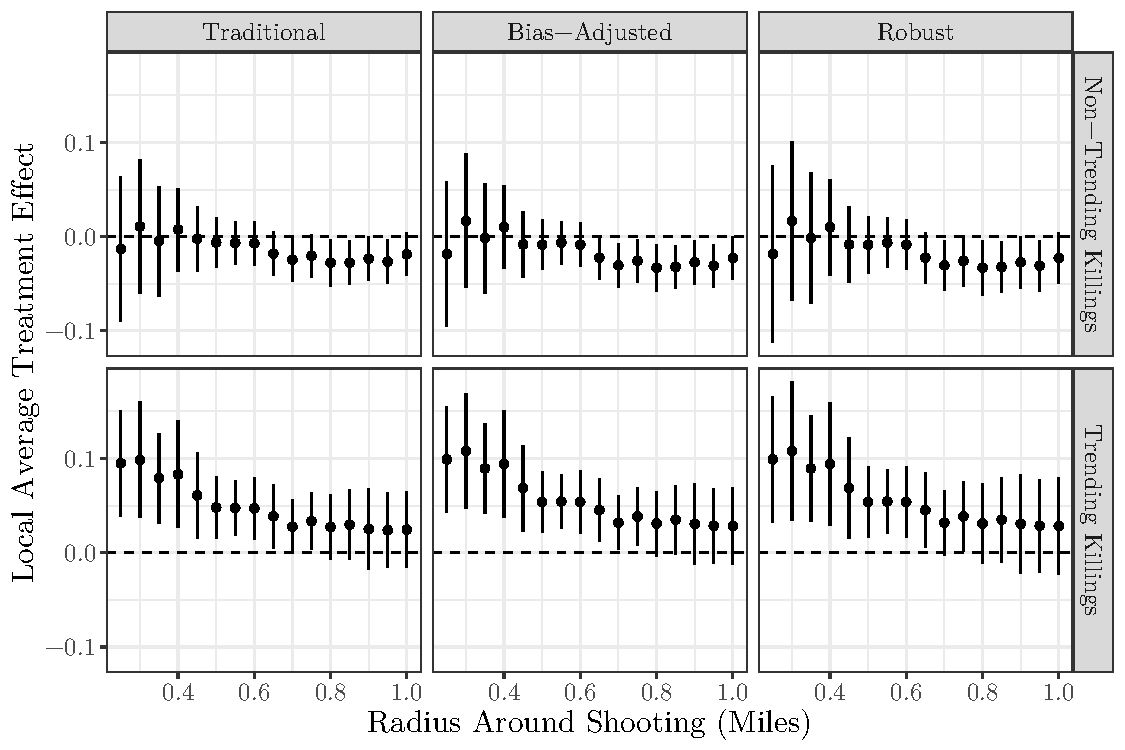
\includegraphics{shoot_to_files/figure-latex/trend-1} 

}

\caption{\label{fig:map}Police Killing within 2 Months of Election, 2016 and 2020}\label{fig:trend}
\end{figure}

\begin{figure}[h]

{\centering 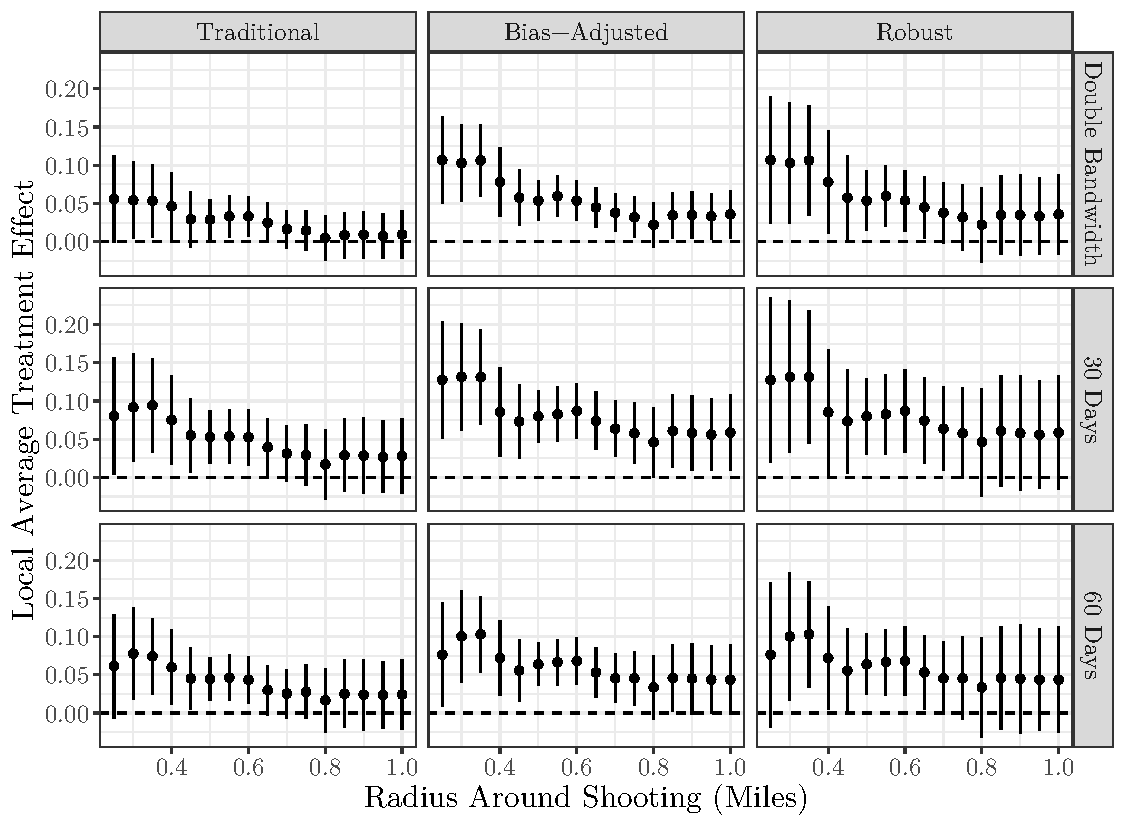
\includegraphics{shoot_to_files/figure-latex/bws-1} 

}

\caption{\label{fig:map}Police Killing within 2 Months of Election, 2016 and 2020}\label{fig:bws}
\end{figure}

\begin{figure}[h]

{\centering 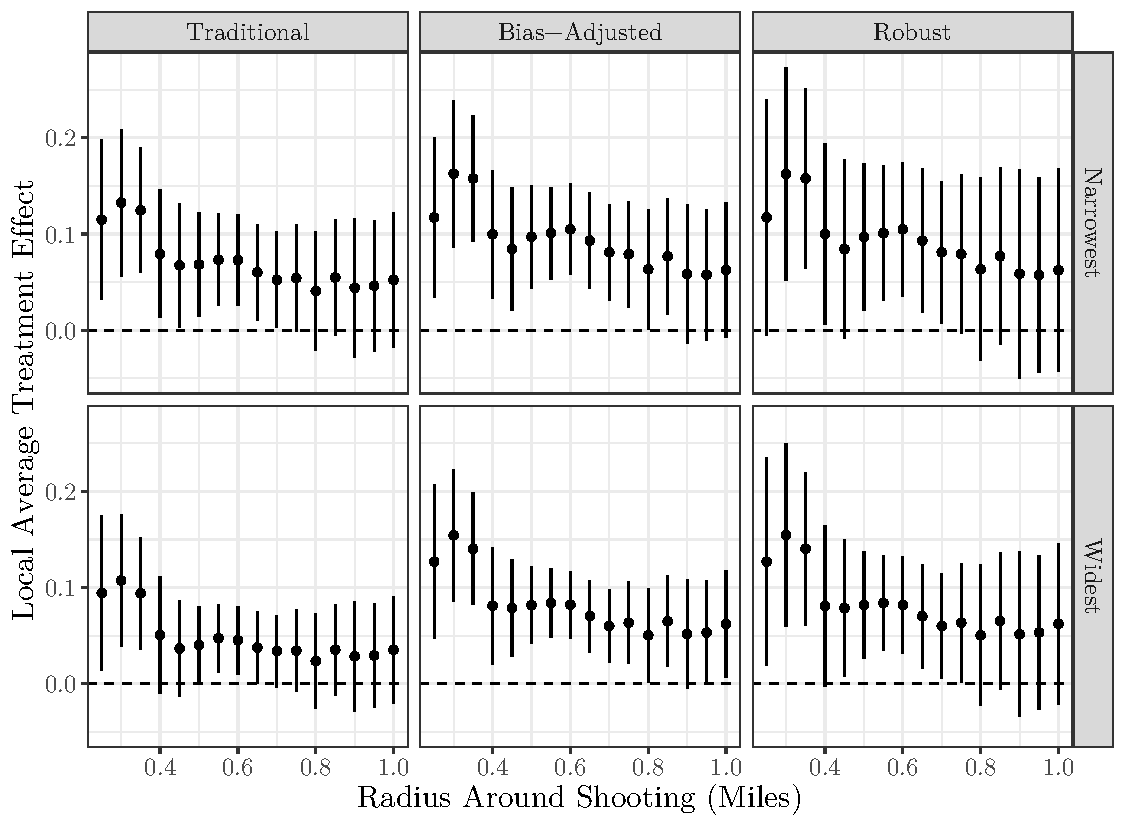
\includegraphics{shoot_to_files/figure-latex/bws-2-1} 

}

\caption{\label{fig:map}Police Killing within 2 Months of Election, 2016 and 2020}\label{fig:bws-2}
\end{figure}

\begin{figure}[h]

{\centering 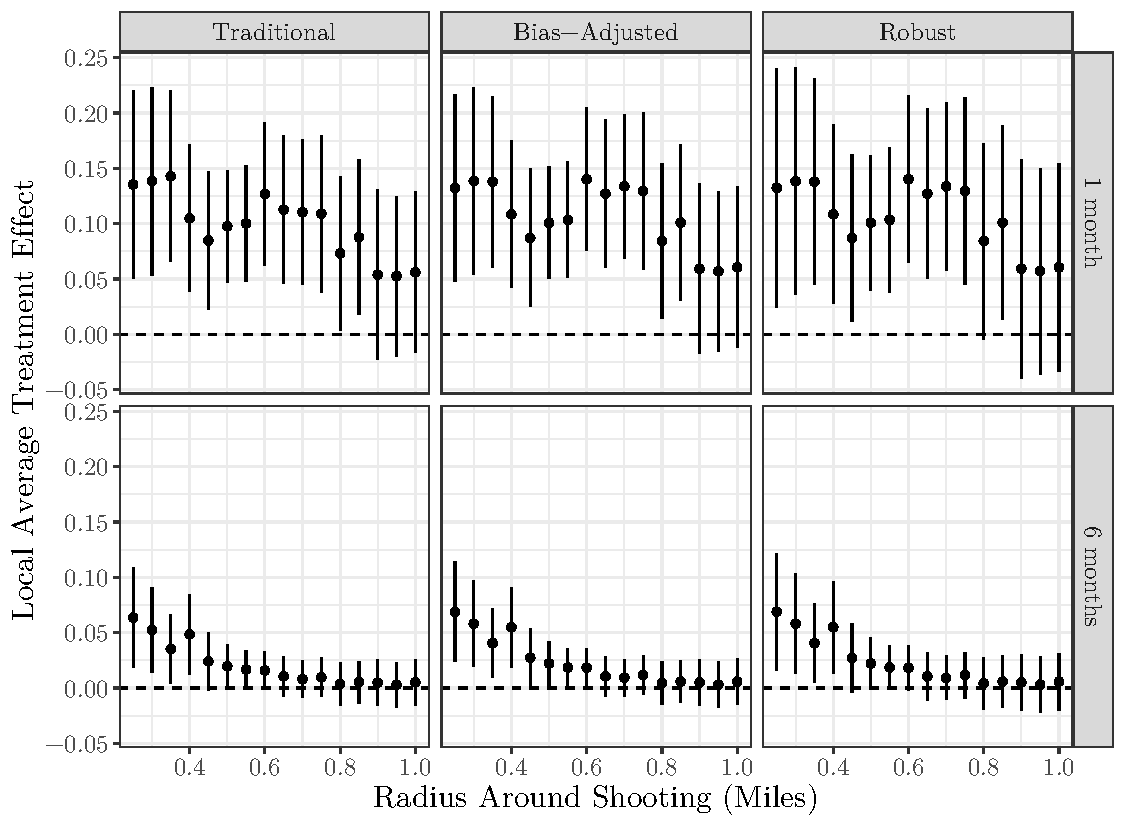
\includegraphics{shoot_to_files/figure-latex/bws-4-1} 

}

\caption{\label{fig:map}Police Killing within 2 Months of Election, 2016 and 2020}\label{fig:bws-4}
\end{figure}

\begin{figure}[h]

{\centering 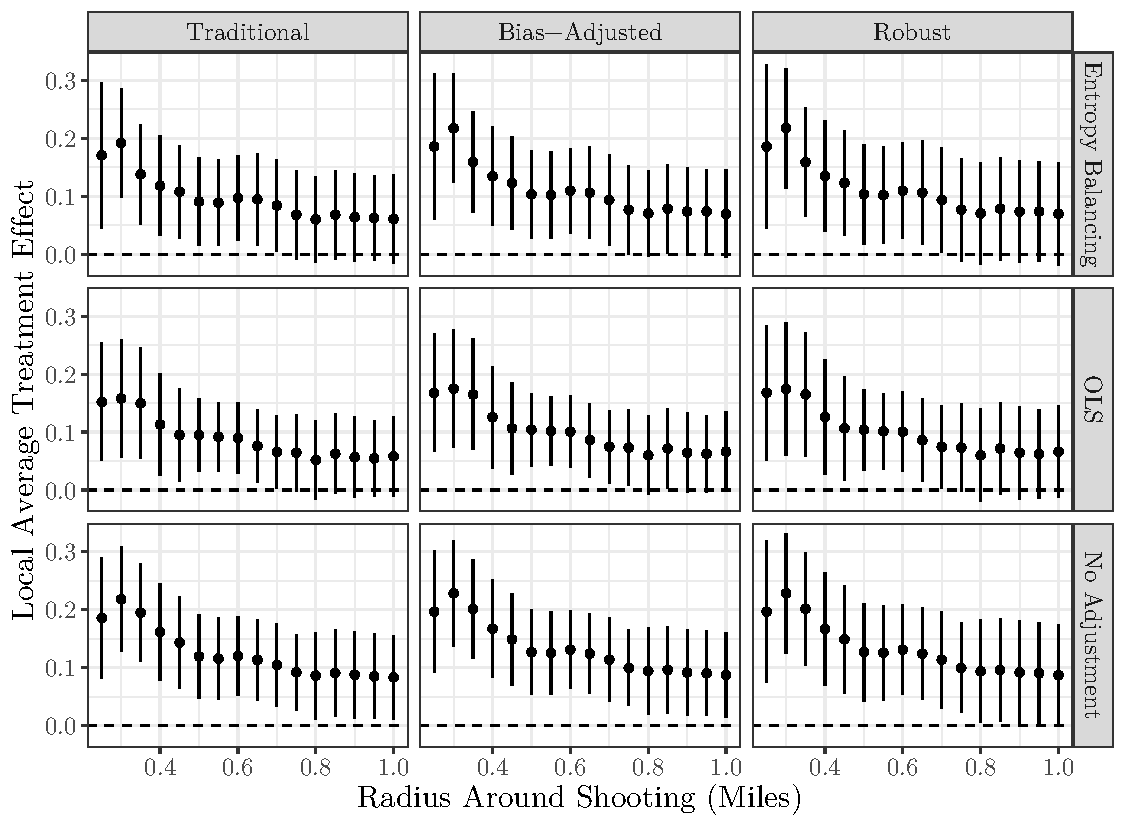
\includegraphics{shoot_to_files/figure-latex/alt-proc-1} 

}

\caption{\label{fig:map}Police Killing within 2 Months of Election, 2016 and 2020}\label{fig:alt-proc}
\end{figure}

\begin{figure}[h]

{\centering 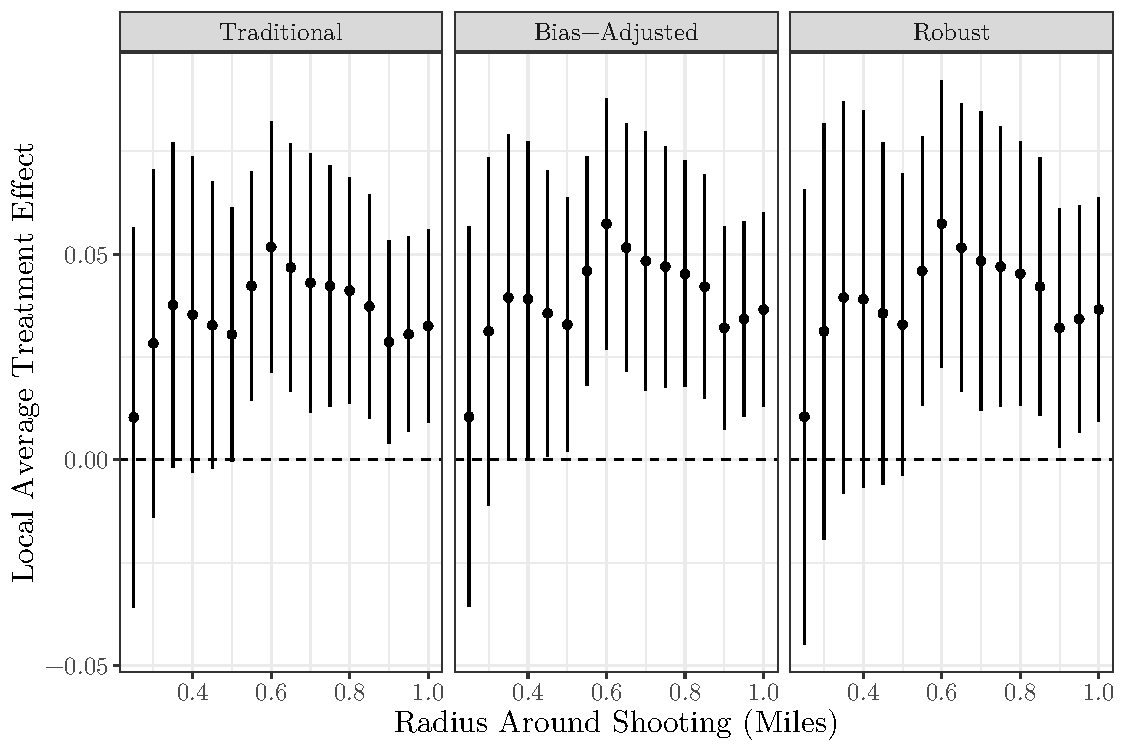
\includegraphics{shoot_to_files/figure-latex/placebo-prior-1} 

}

\caption{\label{fig:map}Police Killing within 2 Months of Election, 2016 and 2020}\label{fig:placebo-prior}
\end{figure}

\begin{figure}[h]

{\centering 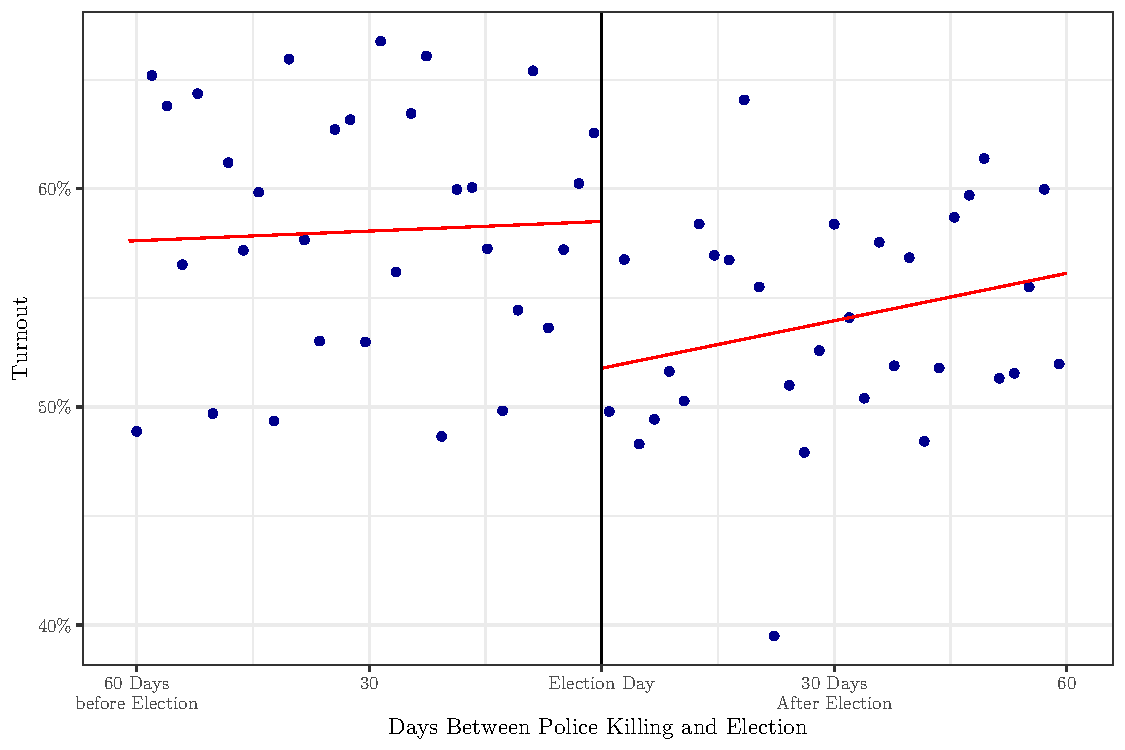
\includegraphics{shoot_to_files/figure-latex/rd-plot-1} 

}

\caption{\label{fig:map}Police Killing within 2 Months of Election, 2016 and 2020}\label{fig:rd-plot}
\end{figure}

\begin{figure}[h]

{\centering 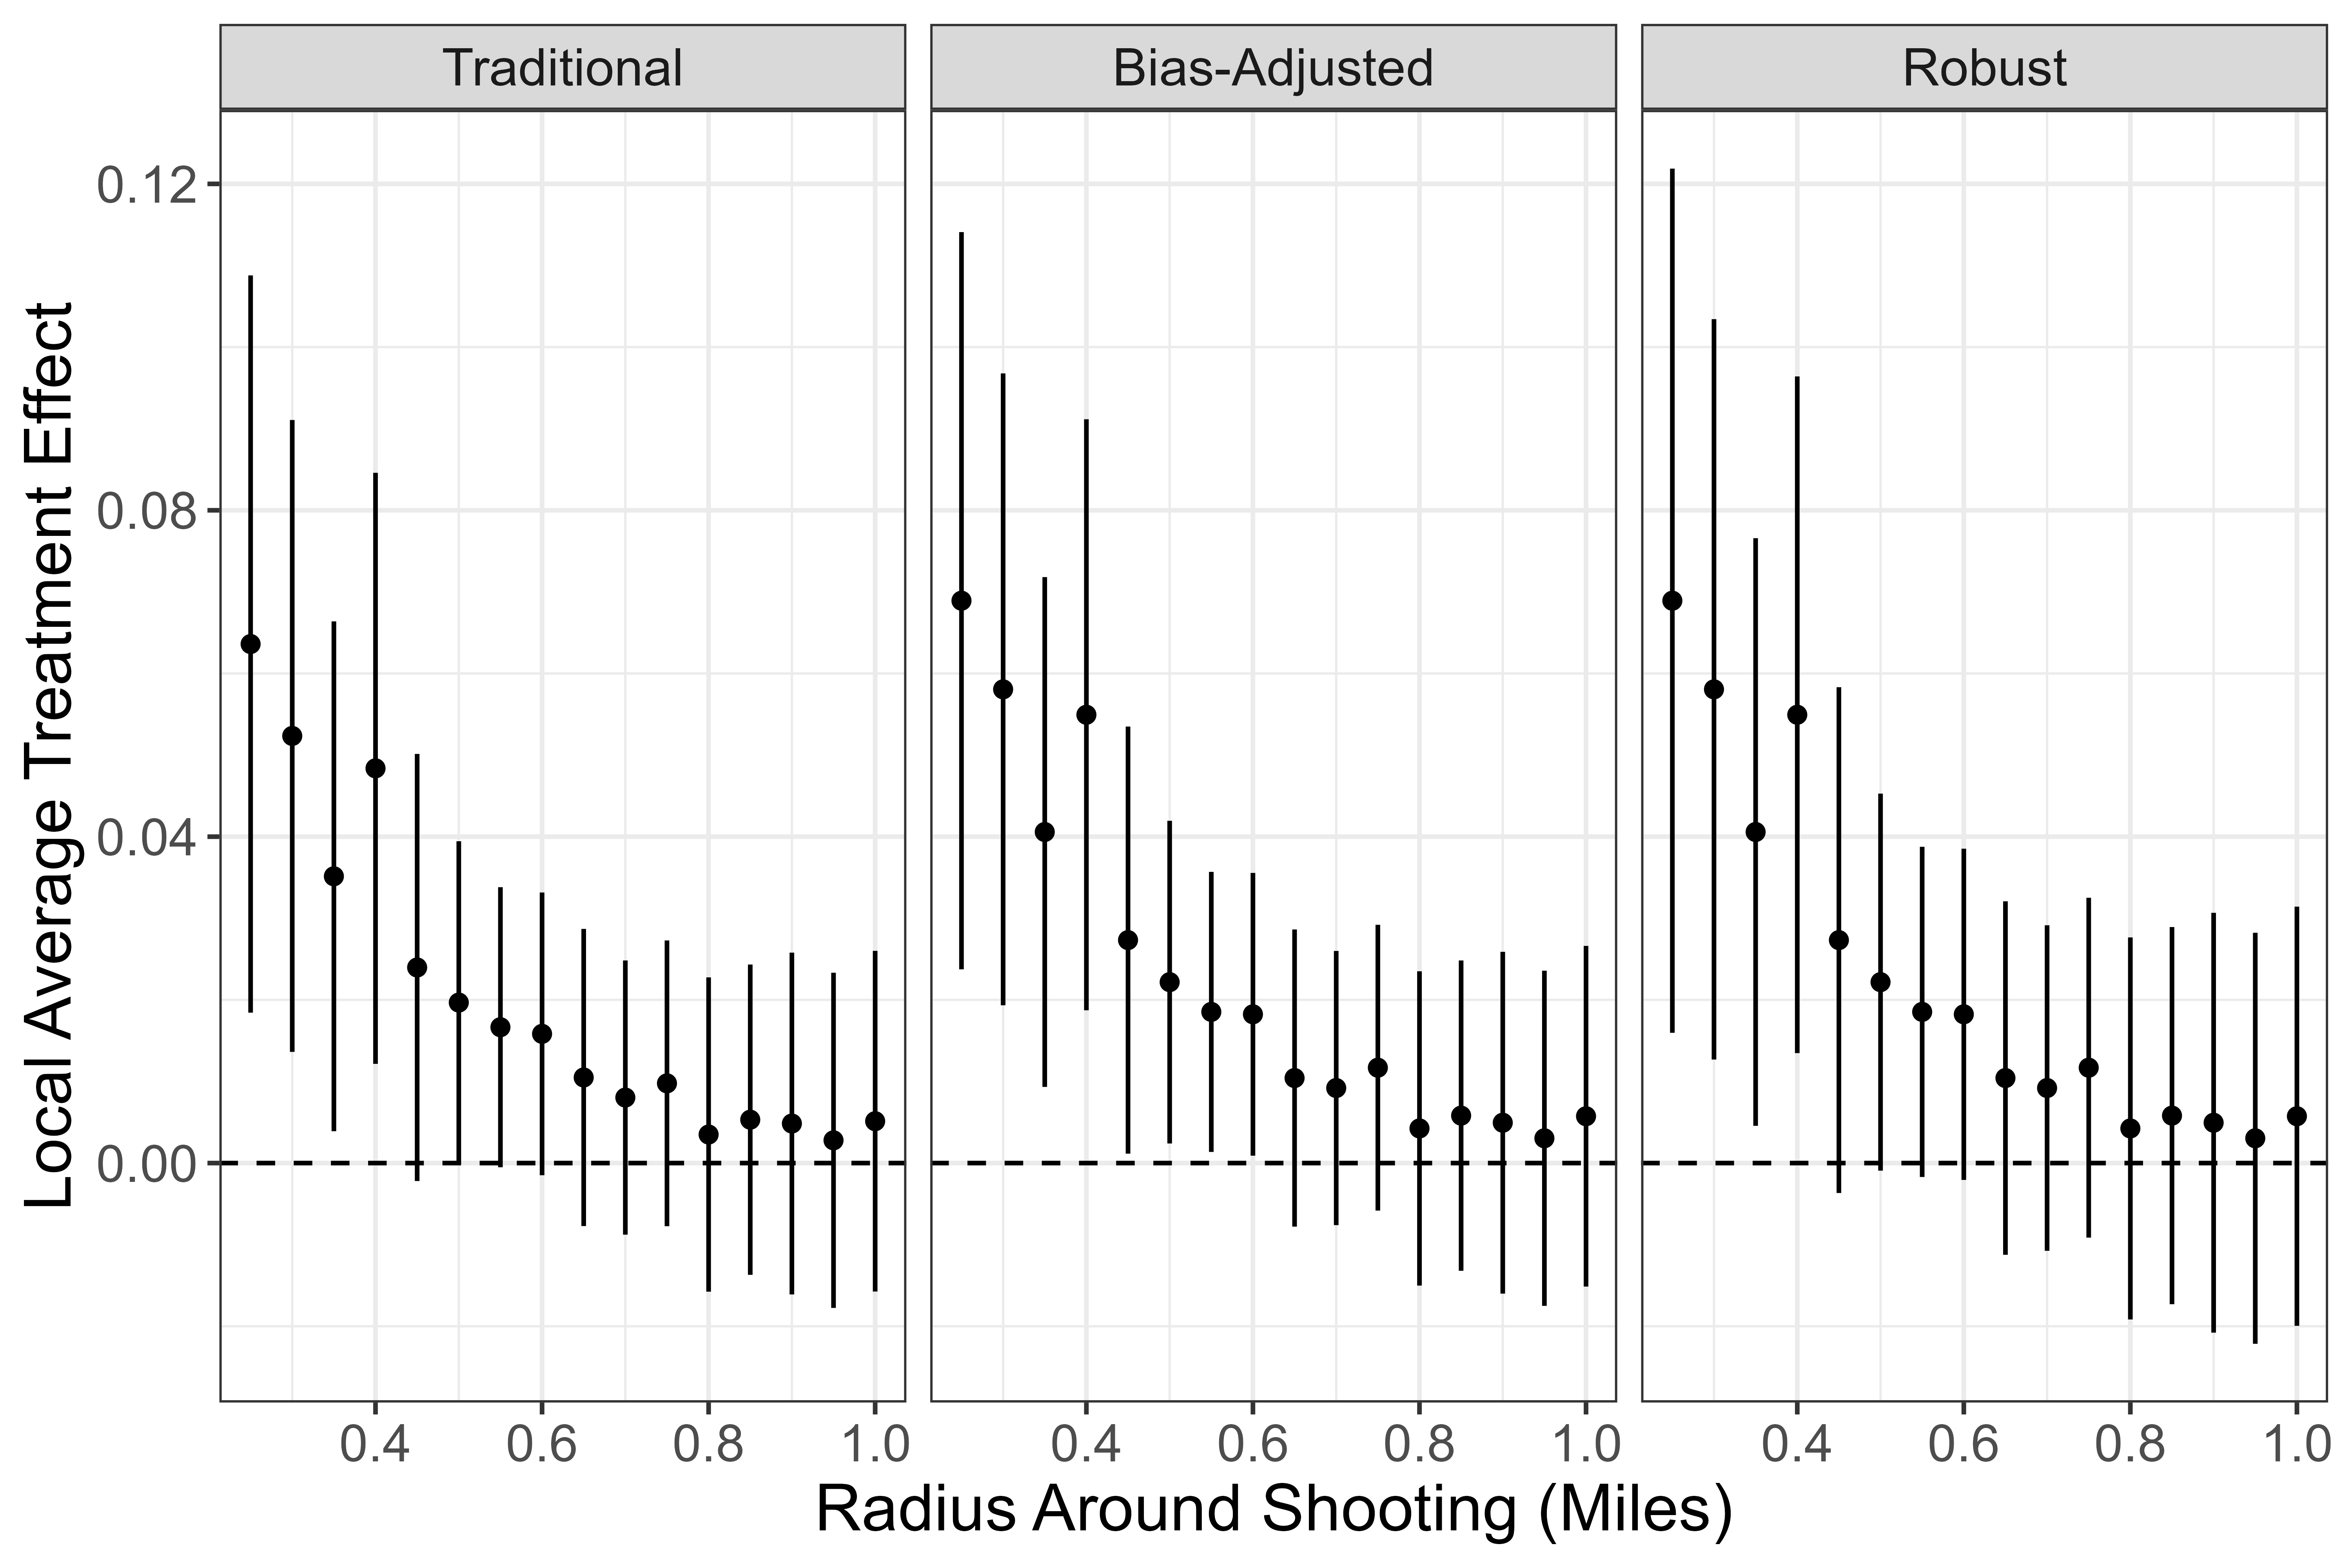
\includegraphics{shoot_to_files/figure-latex/dists-1} 

}

\caption{\label{fig:map}Police Killing within 2 Months of Election, 2016 and 2020}\label{fig:dists}
\end{figure}

\begin{figure}[h]

{\centering 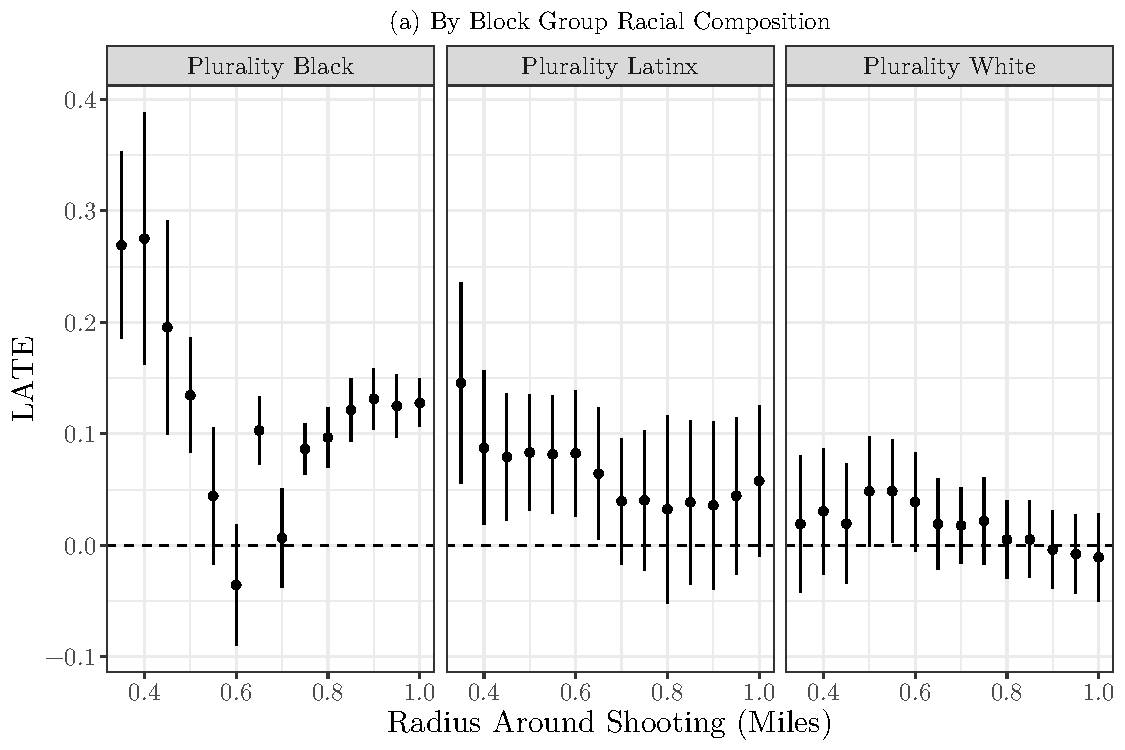
\includegraphics{shoot_to_files/figure-latex/nhood-1} 

}

\caption{\label{fig:map}Police Killing within 2 Months of Election, 2016 and 2020}\label{fig:nhood}
\end{figure}

\begin{figure}[h]

{\centering 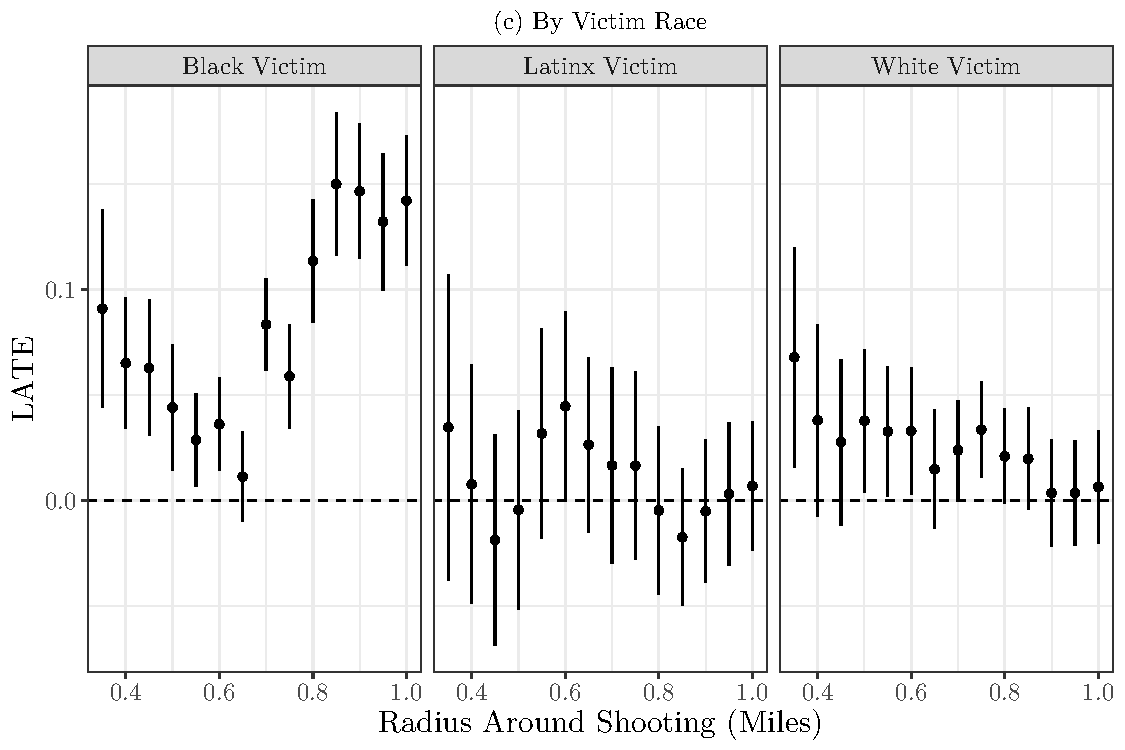
\includegraphics{shoot_to_files/figure-latex/victim-1} 

}

\caption{\label{fig:map}Police Killing within 2 Months of Election, 2016 and 2020}\label{fig:victim}
\end{figure}

\begin{figure}[h]

{\centering 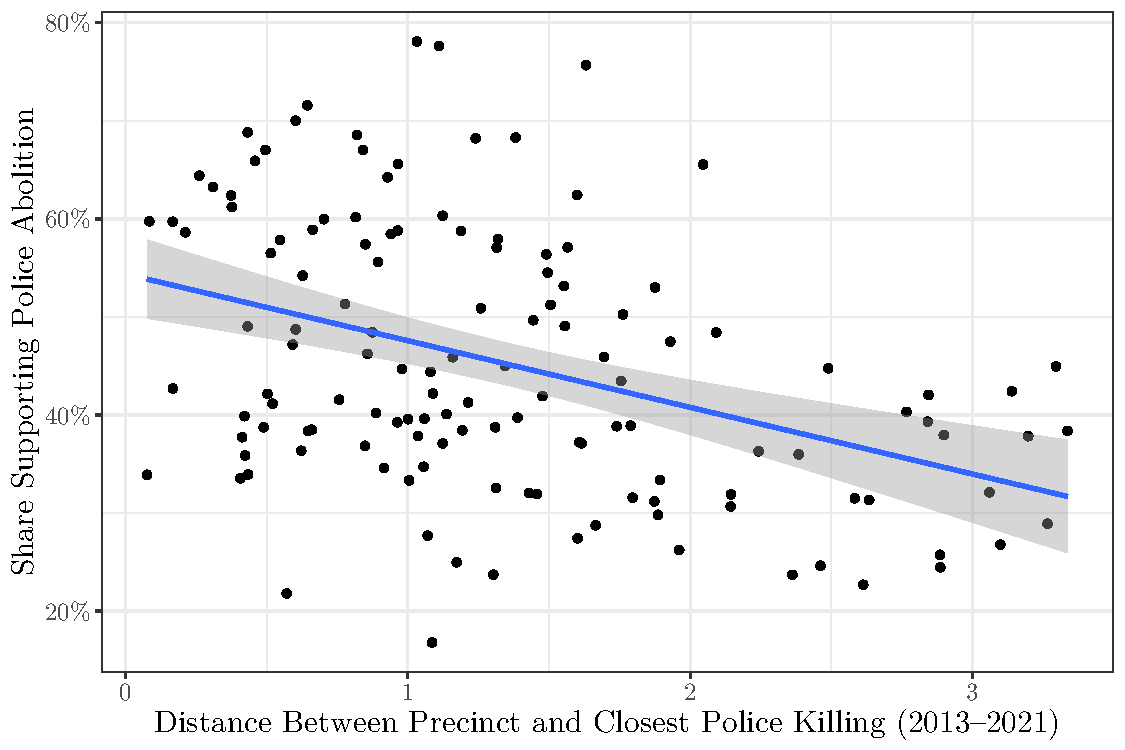
\includegraphics{shoot_to_files/figure-latex/minn-scatter-1} 

}

\caption{\label{fig:map}Police Killing within 2 Months of Election, 2016 and 2020}\label{fig:minn-scatter}
\end{figure}

\begin{figure}[h]

{\centering 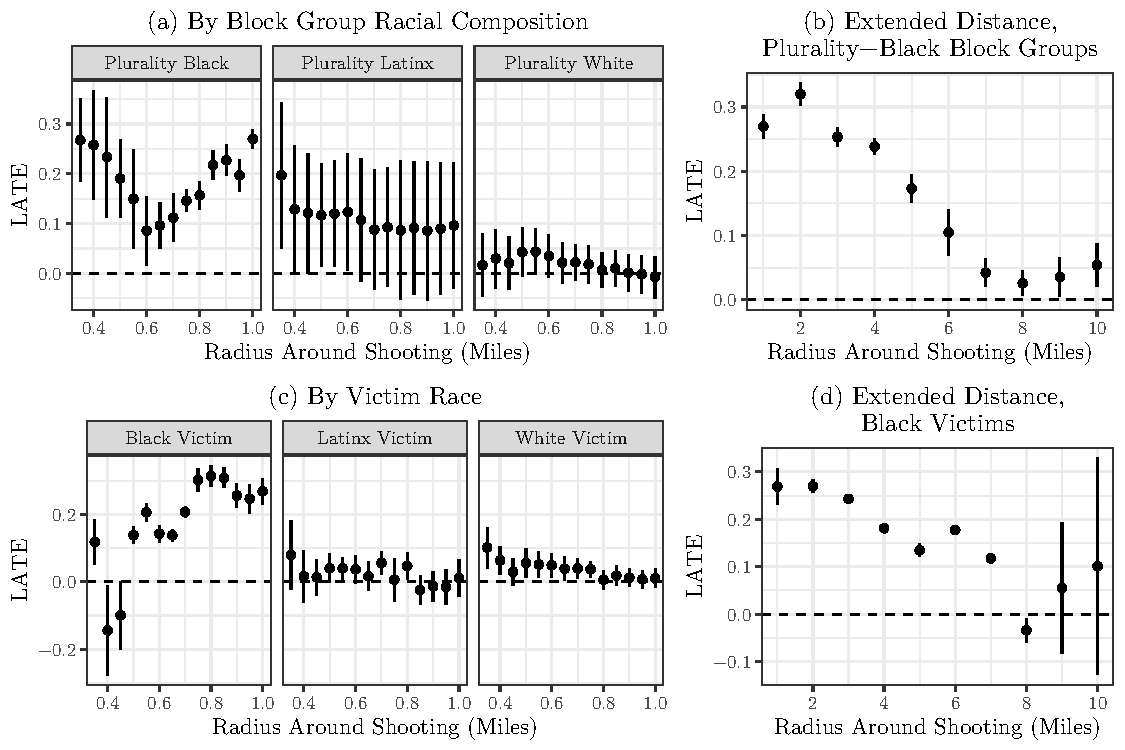
\includegraphics{shoot_to_files/figure-latex/paneled-race-effects-1} 

}

\caption{\label{fig:map}Police Killing within 2 Months of Election, 2016 and 2020}\label{fig:paneled-race-effects}
\end{figure}

\begin{figure}[h]

{\centering 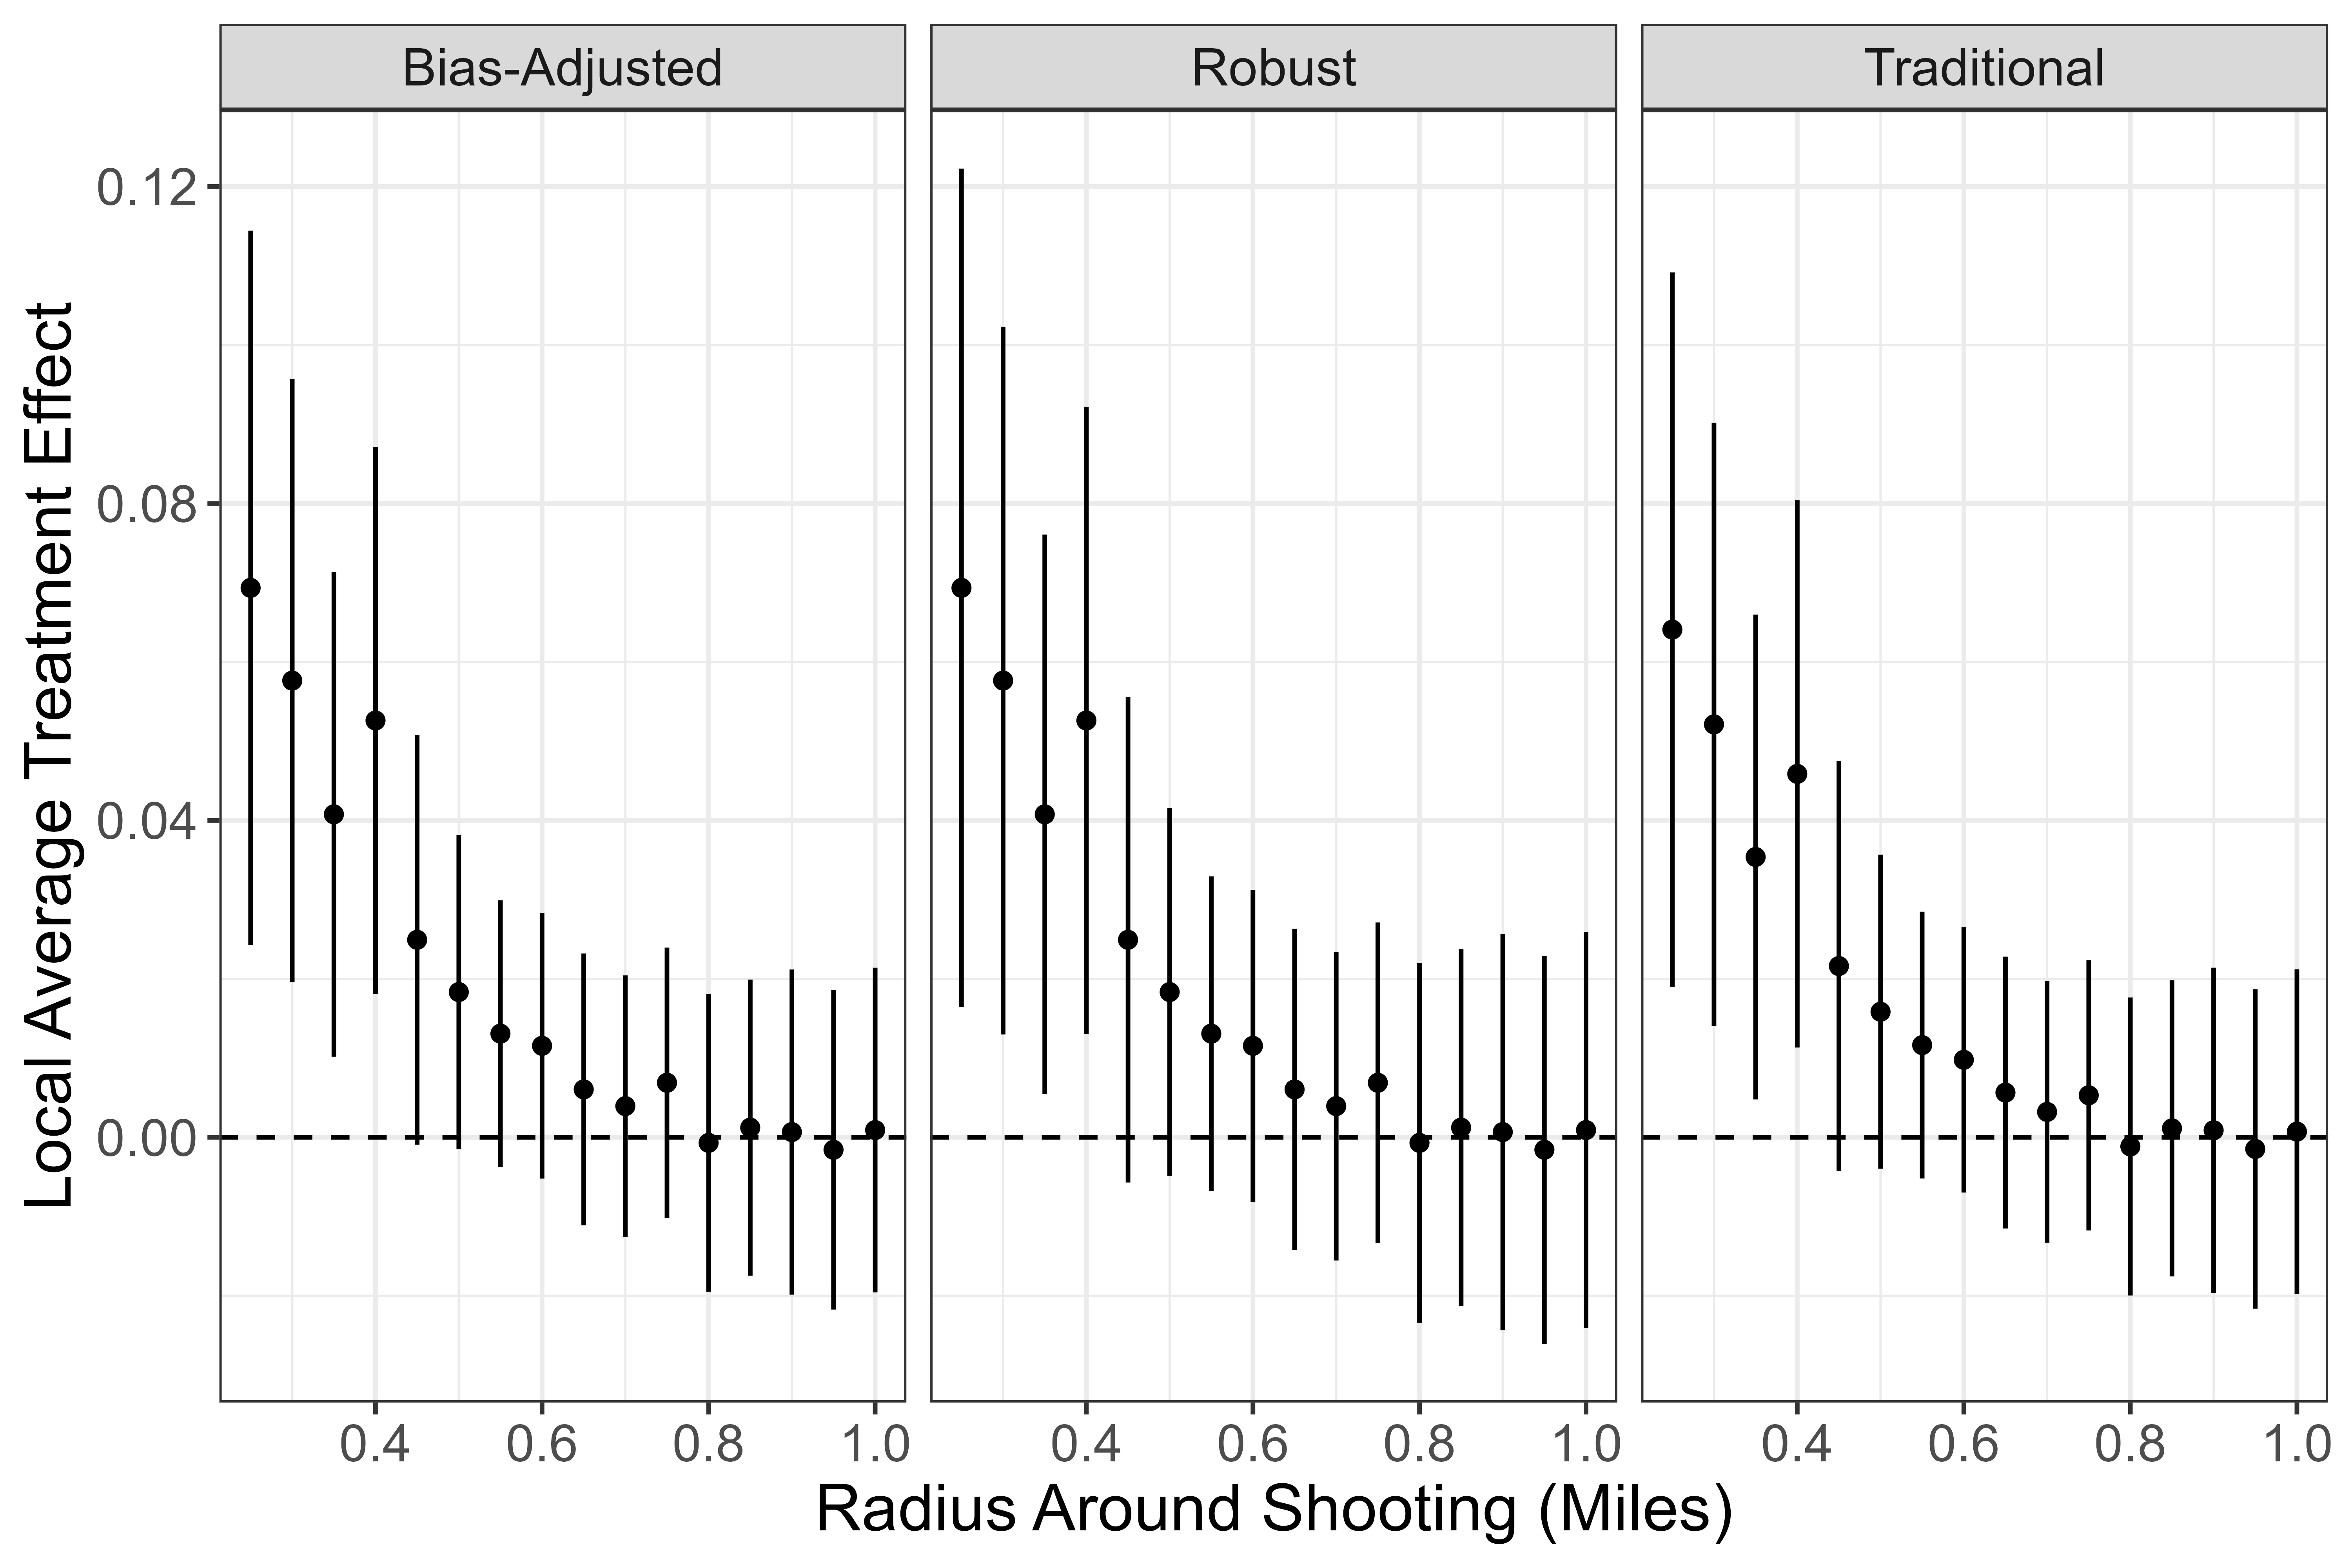
\includegraphics{shoot_to_files/figure-latex/first-difference-1} 

}

\caption{\label{fig:map}Police Killing within 2 Months of Election, 2016 and 2020}\label{fig:first-difference}
\end{figure}

\begin{figure}[h]

{\centering 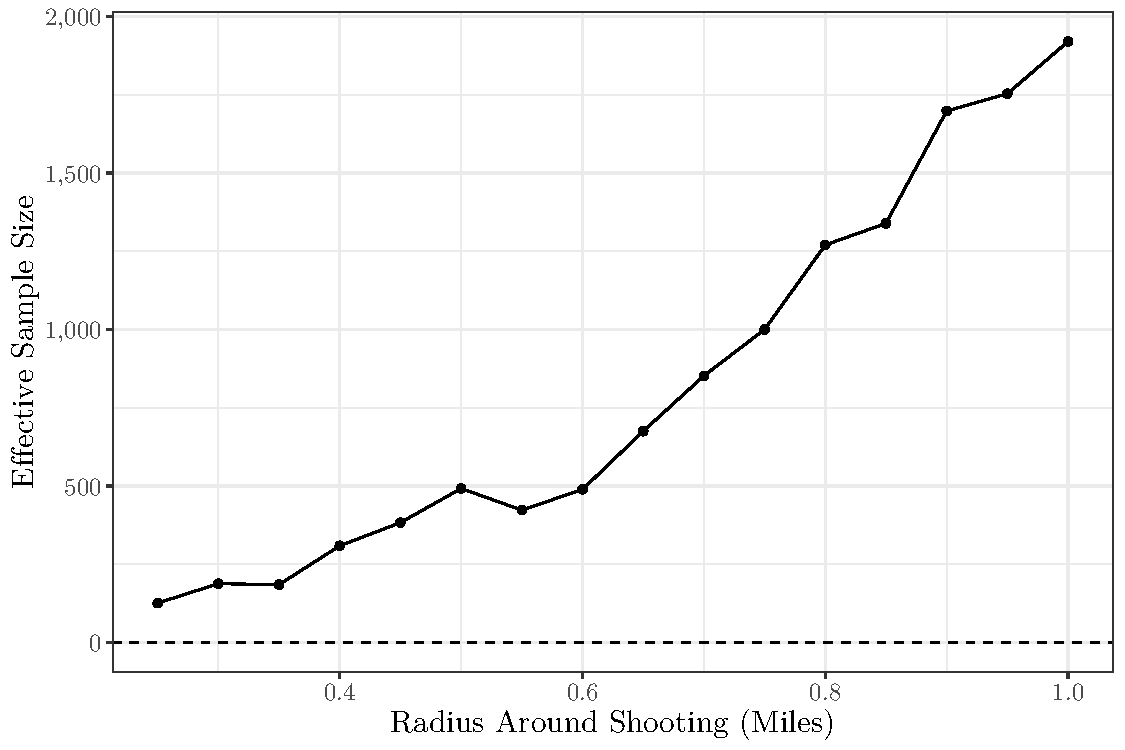
\includegraphics{shoot_to_files/figure-latex/samples-1} 

}

\caption{\label{fig:map}Police Killing within 2 Months of Election, 2016 and 2020}\label{fig:samples}
\end{figure}

\begin{figure}[h]

{\centering 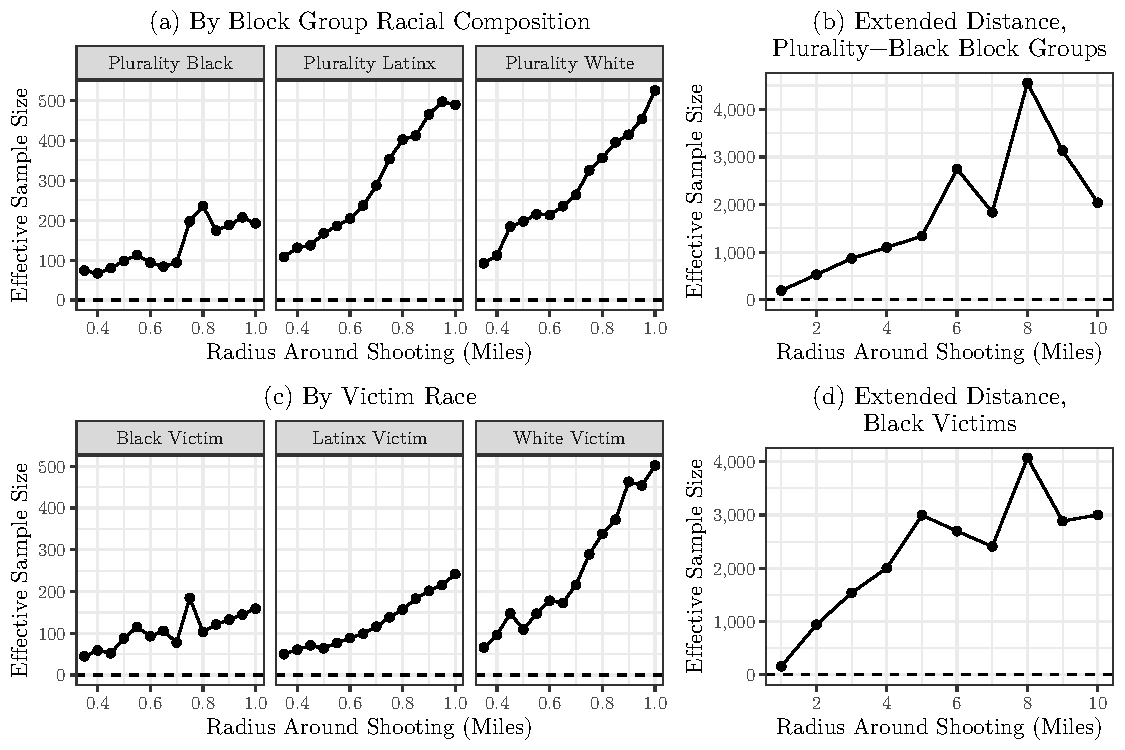
\includegraphics{shoot_to_files/figure-latex/samples-bo-1} 

}

\caption{\label{fig:map}Police Killing within 2 Months of Election, 2016 and 2020}\label{fig:samples-bo}
\end{figure}

\begin{figure}[h]

{\centering 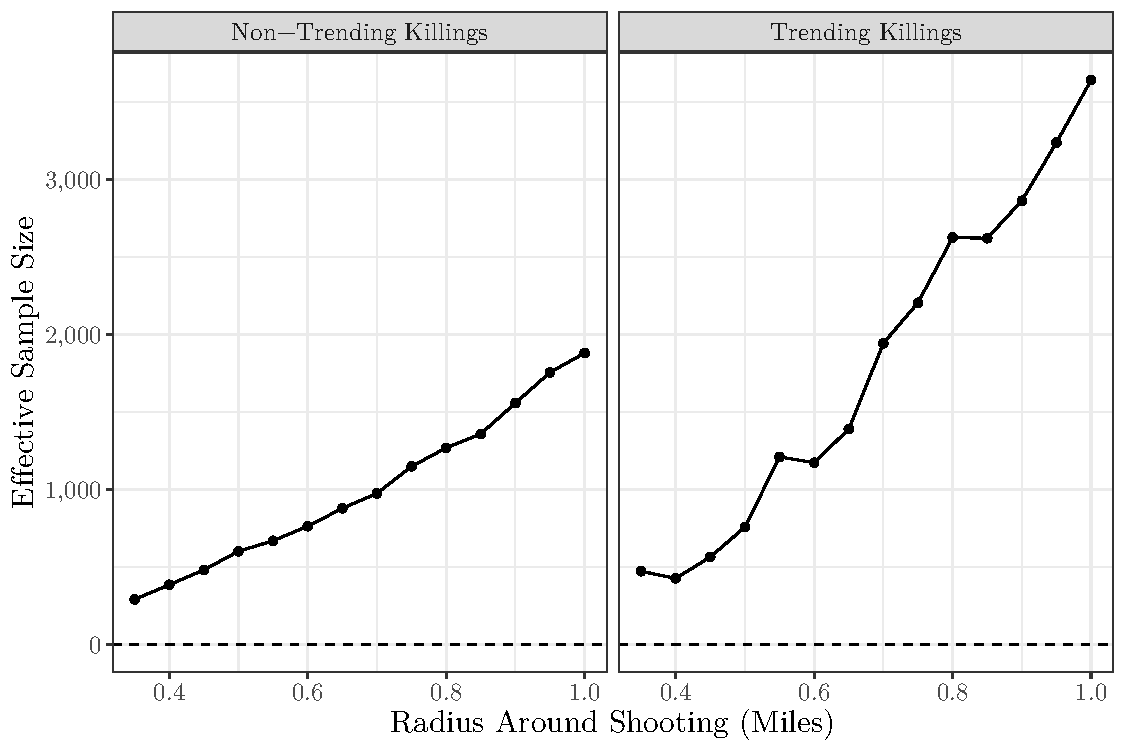
\includegraphics{shoot_to_files/figure-latex/samples-trend-1} 

}

\caption{\label{fig:map}Police Killing within 2 Months of Election, 2016 and 2020}\label{fig:samples-trend}
\end{figure}

\begin{figure}[h]

{\centering 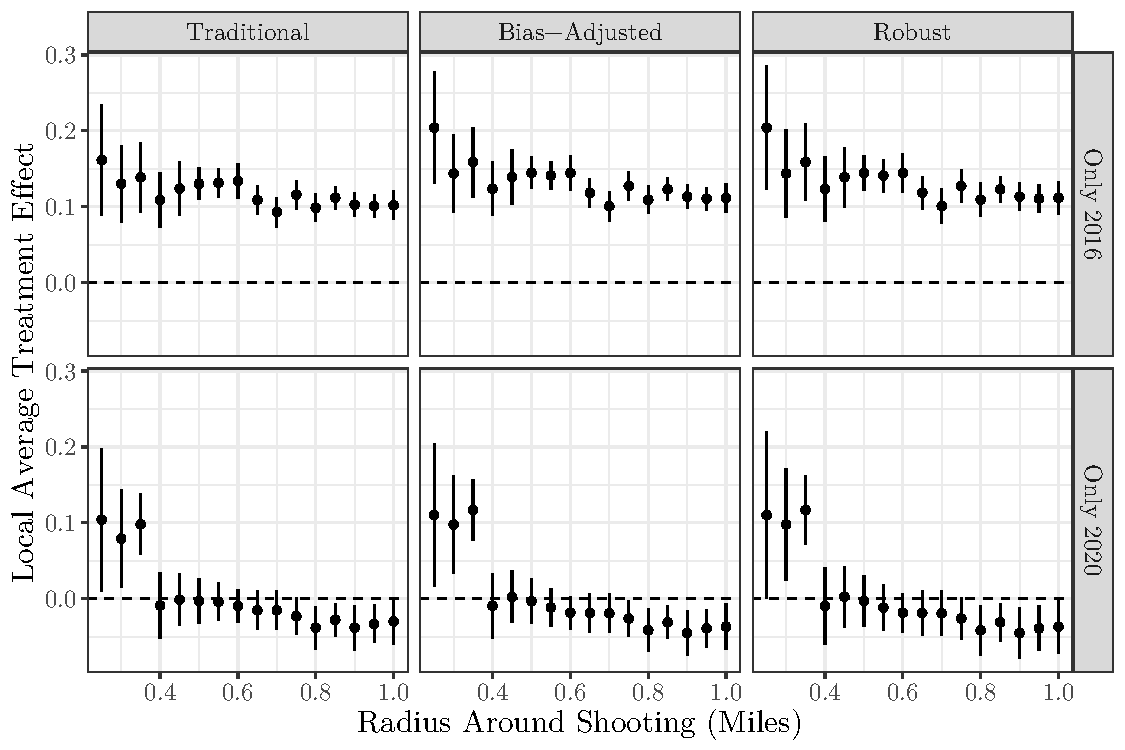
\includegraphics{shoot_to_files/figure-latex/individ-years-1} 

}

\caption{\label{fig:map}Police Killing within 2 Months of Election, 2016 and 2020}\label{fig:individ-years}
\end{figure}

\begin{singlespace}

 
\begin{table}[H]

\caption{\label{tab:balance-tab-full}\label{tab:full-bal} Demographics of Block Groups with Police Killings}
\centering
\begin{tabular}[t]{l>{\raggedright\arraybackslash}p{1in}>{\raggedright\arraybackslash}p{1in}>{\raggedright\arraybackslash}p{1in}>{\raggedright\arraybackslash}p{1in}}
\toprule
 & Not in Dataset & Treated & Unweighted Controls & Weighted Controls\\
\midrule
\addlinespace[0.3em]
\multicolumn{5}{l}{\textbf{2016}}\\
\hspace{1em}\% White & 64.3\% & 33.4\% & 30.6\% & 33.4\%\\
\hspace{1em}\% Black & 12.7\% & 22.1\% & 28.7\% & 22.1\%\\
\hspace{1em}\% Latino & 15.4\% & 34.0\% & 30.5\% & 34.0\%\\
\hspace{1em}\% Asian & 4.5\% & 6.8\% & 6.7\% & 6.8\%\\
\hspace{1em}Median Age & 40 & 35.2 & 35.2 & 35.2\\
\hspace{1em}\% with Some College & 57.9\% & 49.9\% & 48.6\% & 49.9\%\\
\hspace{1em}Median Income & \$60,890 & \$46,466 & \$45,362 & \$46,466\\
\hspace{1em}Population Density & 6,212 & 17,438 & 20,552 & 17,438\\
\hspace{1em}Previous Turnout & 35.9\% & 26.8\% & 25.5\% & 26.8\%\\
\hspace{1em}Number of Block Groups & 209,558 & 426 & 500 & 500\\
\hspace{1em}Number of Killings & 0 & 237 & 236 & 236\\
\addlinespace[0.3em]
\multicolumn{5}{l}{\textbf{2020}}\\
\hspace{1em}\% White & 62.9\% & 36.1\% & 30.5\% & 36.1\%\\
\hspace{1em}\% Black & 12.7\% & 17.9\% & 25.5\% & 17.9\%\\
\hspace{1em}\% Latino & 16.2\% & 36.4\% & 34.3\% & 36.4\%\\
\hspace{1em}\% Asian & 4.8\% & 6.0\% & 6.1\% & 6.0\%\\
\hspace{1em}Median Age & 40.6 & 36.2 & 35.9 & 36.2\\
\hspace{1em}\% with Some College & 59.6\% & 52.1\% & 49.8\% & 52.1\%\\
\hspace{1em}Median Income & \$69,322 & \$53,930 & \$51,360 & \$53,930\\
\hspace{1em}Population Density & 6,271 & 18,585 & 22,646 & 18,585\\
\hspace{1em}Previous Turnout & 49.6\% & 42.2\% & 38.5\% & 42.2\%\\
\hspace{1em}Number of Block Groups & 205,224 & 413 & 413 & 413\\
\hspace{1em}Number of Killings & 0 & 243 & 227 & 227\\
\bottomrule
\end{tabular}
\end{table}
\begin{table}[H]

\caption{\label{tab:big-tab}\label{tab:big-tab} RDiT Outcomes, Primary Model}
\centering
\begin{tabular}[t]{llrlrlr}
\toprule
Threshold (Miles) & Type & RD Estimate & Effective Sample Size & p-value & Confidence
Interval & Std. Error\\
\midrule
0.25 & Traditional & 0.064 & 308 & 0.006 & {}[0.018, 0.109] & 0.023\\
 & Bias-Adjusted & 0.069 & 308 & 0.003 & {}[0.024, 0.114] & 0.023\\
 & Robust & 0.069 & 308 & 0.011 & {}[0.016, 0.122] & 0.027\\
0.3 & Traditional & 0.052 & 528 & 0.008 & {}[0.014, 0.091] & 0.020\\
 & Bias-Adjusted & 0.058 & 528 & 0.003 & {}[0.019, 0.097] & 0.020\\
 & Robust & 0.058 & 528 & 0.012 & {}[0.013, 0.103] & 0.023\\
0.35 & Traditional & 0.035 & 798 & 0.027 & {}[0.004, 0.066] & 0.016\\
 & Bias-Adjusted & 0.041 & 798 & 0.011 & {}[0.009, 0.072] & 0.016\\
 & Robust & 0.041 & 798 & 0.027 & {}[0.005, 0.077] & 0.018\\
0.4 & Traditional & 0.048 & 702 & 0.009 & {}[0.012, 0.085] & 0.018\\
 & Bias-Adjusted & 0.055 & 702 & 0.003 & {}[0.019, 0.091] & 0.018\\
 & Robust & 0.055 & 702 & 0.009 & {}[0.013, 0.096] & 0.021\\
0.45 & Traditional & 0.024 & 1,069 & 0.073 & {}[-0.002, 0.05] & 0.013\\
 & Bias-Adjusted & 0.027 & 1,069 & 0.041 & {}[0.001, 0.053] & 0.013\\
 & Robust & 0.027 & 1,069 & 0.084 & {}[-0.004, 0.058] & 0.016\\
0.5 & Traditional & 0.020 & 1,363 & 0.051 & {}[0, 0.039] & 0.010\\
 & Bias-Adjusted & 0.022 & 1,363 & 0.028 & {}[0.002, 0.042] & 0.010\\
 & Robust & 0.022 & 1,363 & 0.060 & {}[-0.001, 0.045] & 0.012\\
0.55 & Traditional & 0.017 & 2,298 & 0.057 & {}[-0.001, 0.034] & 0.009\\
 & Bias-Adjusted & 0.019 & 2,298 & 0.034 & {}[0.001, 0.036] & 0.009\\
 & Robust & 0.019 & 2,298 & 0.073 & {}[-0.002, 0.039] & 0.010\\
0.6 & Traditional & 0.016 & 2,556 & 0.073 & {}[-0.001, 0.033] & 0.009\\
 & Bias-Adjusted & 0.018 & 2,556 & 0.039 & {}[0.001, 0.036] & 0.009\\
 & Robust & 0.018 & 2,556 & 0.078 & {}[-0.002, 0.039] & 0.010\\
0.65 & Traditional & 0.010 & 2,608 & 0.259 & {}[-0.008, 0.029] & 0.009\\
 & Bias-Adjusted & 0.010 & 2,608 & 0.262 & {}[-0.008, 0.029] & 0.009\\
 & Robust & 0.010 & 2,608 & 0.346 & {}[-0.011, 0.032] & 0.011\\
0.7 & Traditional & 0.008 & 3,489 & 0.349 & {}[-0.009, 0.025] & 0.009\\
 & Bias-Adjusted & 0.009 & 3,489 & 0.283 & {}[-0.008, 0.026] & 0.009\\
 & Robust & 0.009 & 3,489 & 0.366 & {}[-0.011, 0.029] & 0.010\\
0.75 & Traditional & 0.010 & 3,926 & 0.274 & {}[-0.008, 0.027] & 0.009\\
 & Bias-Adjusted & 0.012 & 3,926 & 0.191 & {}[-0.006, 0.029] & 0.009\\
 & Robust & 0.012 & 3,926 & 0.271 & {}[-0.009, 0.033] & 0.011\\
0.8 & Traditional & 0.003 & 4,515 & 0.722 & {}[-0.016, 0.023] & 0.010\\
 & Bias-Adjusted & 0.004 & 4,515 & 0.666 & {}[-0.015, 0.024] & 0.010\\
 & Robust & 0.004 & 4,515 & 0.722 & {}[-0.019, 0.028] & 0.012\\
0.85 & Traditional & 0.005 & 5,031 & 0.584 & {}[-0.014, 0.024] & 0.010\\
 & Bias-Adjusted & 0.006 & 5,031 & 0.549 & {}[-0.013, 0.025] & 0.010\\
 & Robust & 0.006 & 5,031 & 0.622 & {}[-0.017, 0.029] & 0.012\\
0.9 & Traditional & 0.005 & 5,604 & 0.650 & {}[-0.016, 0.026] & 0.011\\
 & Bias-Adjusted & 0.005 & 5,604 & 0.644 & {}[-0.016, 0.026] & 0.011\\
 & Robust & 0.005 & 5,604 & 0.706 & {}[-0.021, 0.031] & 0.013\\
0.95 & Traditional & 0.003 & 6,102 & 0.790 & {}[-0.018, 0.023] & 0.010\\
 & Bias-Adjusted & 0.003 & 6,102 & 0.772 & {}[-0.017, 0.024] & 0.010\\
 & Robust & 0.003 & 6,102 & 0.813 & {}[-0.022, 0.028] & 0.013\\
1 & Traditional & 0.005 & 6,799 & 0.630 & {}[-0.016, 0.026] & 0.011\\
 & Bias-Adjusted & 0.006 & 6,799 & 0.590 & {}[-0.015, 0.027] & 0.011\\
 & Robust & 0.006 & 6,799 & 0.661 & {}[-0.02, 0.031] & 0.013\\
\bottomrule
\end{tabular}
\end{table}
 
\end{singlespace}

\end{document}
